\documentclass[twoside]{article}
\usepackage[accepted]{aistats2017}
\usepackage[round]{natbib}
\usepackage{listings}
\usepackage{minted}
\usepackage{color}
\usepackage{algorithm}
\usepackage{algpseudocode}
\usepackage{amsmath}
\usepackage{amssymb}
\usepackage{dsfont}
\usepackage{pgf}
\usepackage{subcaption}
\usepackage{tikz}
\usetikzlibrary{bayesnet}
%\graphicspath{{report_data_and_plots/}}
%\definecolor{mygreen}{rgb}{0,0.6,0}
%\definecolor{mygray}{rgb}{0.5,0.5,0.5}
%\definecolor{mymauve}{rgb}{0.58,0,0.82}
%
%\lstset{ %
%	backgroundcolor=\color{white},   % choose the background color; you must add \usepackage{color} or \usepackage{xcolor}; should come as last argument
%	basicstyle=\footnotesize,        % the size of the fonts that are used for the code
%	breakatwhitespace=false,         % sets if automatic breaks should only happen at whitespace
%	breaklines=true,                 % sets automatic line breaking
%	captionpos=b,                    % sets the caption-position to bottom
%	commentstyle=\color{mygreen},    % comment style
%	deletekeywords={...},            % if you want to delete keywords from the given language
%	escapeinside={\%*}{*)},          % if you want to add LaTeX within your code
%	extendedchars=true,              % lets you use non-ASCII characters; for 8-bits encodings only, does not work with UTF-8
%	frame=single,	                   % adds a frame around the code
%	keepspaces=true,                 % keeps spaces in text, useful for keeping indentation of code (possibly needs columns=flexible)
%	keywordstyle=\color{blue},       % keyword style
%	language=Octave,                 % the language of the code
%	morekeywords={*,...},            % if you want to add more keywords to the set
%	numbers=left,                    % where to put the line-numbers; possible values are (none, left, right)
%	numbersep=5pt,                   % how far the line-numbers are from the code
%	numberstyle=\tiny\color{mygray}, % the style that is used for the line-numbers
%	rulecolor=\color{black},         % if not set, the frame-color may be changed on line-breaks within not-black text (e.g. comments (green here))
%	showspaces=false,                % show spaces everywhere adding particular underscores; it overrides 'showstringspaces'
%	showstringspaces=false,          % underline spaces within strings only
%	showtabs=false,                  % show tabs within strings adding particular underscores
%	stepnumber=2,                    % the step between two line-numbers. If it's 1, each line will be numbered
%	stringstyle=\color{mymauve},     % string literal style
%	tabsize=2,	                   % sets default tabsize to 2 spaces
%%	title=\lstname                   % show the filename of files included with \lstinputlisting; also try caption instead of title
%}
 % If your paper is accepted, change the options for the package
% aistats2017 as follows:
%
%\usepackage[accepted]{aistats2017}
%
% This option will print headings for the title of your paper and
% headings for the authors names, plus a copyright note at the end of
% the first column of the first page.

\renewcommand{\bibsection}{}
\begin{document}

% If your paper is accepted and the title of your paper is very long,
% the style will print as headings an error message. Use the following
% command to supply a shorter title of your paper so that it can be
% used as headings.
%
%\runningtitle{I use this title instead because the last one was very long}

% If your paper is accepted and the number of authors is large, the
% style will print as headings an error message. Use the following
% command to supply a shorter version of the authors names so that
% they can be used as headings (for example, use only the surnames)
%
%\runningauthor{Surname 1, Surname 2, Surname 3, ...., Surname n}

\twocolumn[

\aistatstitle{Hamiltonian Monte Carlo Inference for a First Order Probabilistic Programming Language }

%\aistatsauthor{ Bradley Gram-Hansen \And Frank Wood \And  Author 3 }
\aistatsauthor{ Bradley Gram-Hansen \And Frank Wood }
%\aistatsaddress{ Institution 1 \And  Institution 2 \And Institution 3 } ]
\aistatsaddress{ Department of Engineering,  University of Oxford } ]
\begin{abstract}
  The Abstract paragraph should be indented 0.25 inch (1.5 picas) on
  both left and right-hand margins. Use 10~point type, with a vertical
  spacing of 11~points. The {\bf Abstract} heading must be centered,
  bold, and in point size 12. Two line spaces precede the
  Abstract. The Abstract must be limited to one paragraph.
\end{abstract}

\section{Introduction}

%\lstinputlisting[language=Python]{test.py}
%Papers are in 2 columns with the overall line width of 6.75~inches (41~picas). Each column is 3.25~inches wide (19.5~picas).  The space
%between the columns is .25~inches wide (1.5~picas).  The left margin is 1~inch (6~picas).  Use 10~point type with a vertical spacing of
%11~points. Please use US Letter size paper instead of A4.
%
%Paper title is 16~point, caps/lc, bold, centered between 2~horizontal rules.  Top rule is 4~points thick and bottom rule is 1~point thick.
%Allow 1/4~inch space above and below title to rules.

Monte Carlo Markov Chain (MCMC) methods are a set of powerful inference algorithms \citep{berg2008markov} that enable us to evaluate, model and analyze complicated probabilistic models. These include, but are not limited to, areas in machine learning such as Bayesian inference and learning, optimisation for finding the optimal hyper-parameters \citep{andrieu2003introduction} and in natural systems, such as those found in Biology \citep{sorensen2007likelihood} and Physics \citep{duane1987hybrid}. 
However, as the dimensionality of the problem grows many MCMC methods, such as Metropolis-Hastings \citep{hastings1970monte}, rejection and importance sampling,  become ineffective at being able to generate independent samples effectively. This can be overcome in some instances by tuning particular parameters, or by choosing a better proposal distribution, but in practice this cannot always be done. One MCMC method that is able to circumvent this problem is Hamiltonian Monte Carlo (HMC) \citep{neal2011mcmc}\citep{duane1987hybrid}, which takes inspiration from the physical world and uses a dynamical model to generate new proposals. This in turn enables us to explore larger spaces more effectively globally, rather than getting trapped in local regions. \\
Choosing the right inference algorithm is critical for probabilistic programming languages \citep{tolpin2015probabilistic} such as Anglican \citep{wood2014new} and others, where we rely upon accurate inference and sampling procedures to evaluate our programs. Although, in practice there is no one inference or sampling algorithm to rule them all. Thus we rely on a combination of techniques to deal with discrete, finite continuous and infinite continuous parameter spaces (non-parametric models). To analyze more effectively a subset of the problems that Anglican and other higher order probabilistic programming languages (HOPPL) can, such as finite graphs, FOPPL, a first order probabilistic programming language was formed so that we could take advantage of fast inference algorithms, such as HMC.\\
In this work we make two contributions, we introduce a FOPPL compiler that transforms a FOPPL output, a finite graph, into python code that takes advantage of the Automatic differentiation package within Pytorch \citep{pytorch} and an HMC that correctly deals with conditional statements and finite continuous parameters.
In section \ref{sec:foppl} we talk about FOPPL, its syntax and primary use, in section \ref{sec:hmc} we introduce HMC, in section \ref{sec:exampprog} we give examples of FOPPL programs and the results generated through HMC inference. In section \ref{sec:supmat} we provide details of HMC implementation and some examples of the compiled FOPPL output. 
\section{FOPPL}
\label{sec:foppl}
In this section include some stuff about FOPPL, what is it, the syntax etc.  The length of the loops are deterministic and finite, whereas in higher order probabilistic programming languages enable a loop to be unrolled an infinite number of times. Although FOPPL is a reduced subset of HOPPLs, it is still a very felxible and rich language, so that one may define incredibly complicated graphical models, such as neural networks.  enough to describe a whole host of probabilistic models. 
\section{Hamiltonian Monte Carlo}
\label{sec:hmc}
In a top level view HMC is a two step process. In step one, we define a Hamiltonian function in terms of the joint probability distribution of the model that we aim to perform inference on and in step two, HMC proposes new states generated via Hamiltonian dynamics for which we apply Metropolis updates. As the proposals are being generated via a physical process, we are able to comprehensively explore our model space \citep{neal2011mcmc}. This is in part due to certain physical properties of the Hamiltonian itself, that make HMC a very powerful, multi-purpose inference algorithm. Adopting the notation from the machine learning literature, we use $\textbf{x} \in \mathbb{R}^{n \times d}$ to represent the parameters of interest, our latent variables, rather than the typical $\mathbf{\theta}$ and $\textbf{q}$ in the HMC literature. Where $n$ represents the number of parameters of interest and $d$ is the dimension of the system.

The Hamiltonian of a physical system is defined completely in terms of the sets of points $(\textbf{x}, \textbf{p})$, the position and momentum variables respectively. These points span what is called the phase space, which formally is defined as the cotangent bundle $T^{*}\mathcal{M}$ of the configuration space $\mathcal{M}$. Simply put, we can imagine the phase space as a manifold that shows us both how our model evolves, with respect to $\textbf{x}$ and $\textbf{p}$ and how it is constrained in regards to the total energy within the system. Where the total energy of the system is given by the Hamiltonian, $H(\textbf{x},\textbf{p})$. The Hamiltonian is the Legendre transform of the Lagrangian and is formally defined as $
H(\textbf{x}, \textbf{p})  = K(\textbf{p}) + U(\textbf{x})$ where $K(\textbf{p})$ represents our kinetic energy and $U(\textbf{x})$ is the potential energy. The Legendre transform is given by $H(\textbf{x},\textbf{p}) = \sum_{i = 1}^{d}\dot{x}_{i}p_{i} - L(\textbf{x}, \textbf{\.{x}}(\textbf{x}, \textbf{p})) $\footnote{The $\dot{x}$ represents that the variable is being differentiated with respect to time.}.  
Thus, for simplicity, if we set $d = 1$, we can derive Hamilton's equations: 
\begin{equation}
\label{eq:hameq1}
\frac{\partial H}{\partial p} = \dot{x} + p\frac{\partial \dot{x}}{\partial p} - \frac{\partial L}{\partial \dot{x}}\frac{\partial \dot{x}}{\partial p} = \dot{x} 
\end{equation}
and 
\begin{equation}
\label{eq:hameq2}
\frac{\partial H}{\partial x} = p\frac{\partial \dot{x}}{\partial x} - \frac{\partial L}{\partial x} - \frac{\partial L}{\partial \dot{x}}\frac{\partial \dot{x}}{\partial x} = - \frac{\partial L}{\partial x}= -\dot{p}  
\end{equation}
from which we can vectorize for higher dimensions. It should be noted that the derivatives for the Lagrangian $L$, come from the Euler-Lagrange equations $\frac{d}{dt}\left(\frac{\partial L}{d\dot{x}}\right) = \frac{\partial L}{dx}$ and the Lagrangian itself, is just a reformulation of Newtonian mechanics.

Within the HMC framework the positions, $\textbf{x}$, are the variables of interest, but in order to simulate Hamiltonian dynamics properly, for each $\textbf{x}$ we must introduce an auxillary momentum variable $\textbf{p}$. But what form should $\textbf{p}$ take? Typically, $\textbf{p}$ is sampled from a normal distribution $\textbf{p} \sim \mathcal{N}(\textbf{0}, \mathds{1})$, although this need not be the case. In HMC, the potential energy $U(\textbf{x})$ represents the negative log joint distribution of the model and is a key component within the algorithm.  The kinetic energy $K(\textbf{p})$, is typically taken to be the mean field approximation, which corresponds directly to the log of a centered Gaussian distribution $K(\textbf{p}) = \frac{\textbf{p}^{T} \textbf{M}^{-1} \textbf{p}}{2}$, where $\textbf{M}$, the mass matrix, is a symmetric, positive definite and typically diagonal matrix. Although, again we need not choose this form of kinetic energy and in some cases, such as those when we are dealing with discrete parameters, it is actually more beneficial to use a different kinetic function\citep{nishimura2017discontinuous}. Thus, if we are to use the standard kinetic energy, which we do for all our current models, then Hamilton's equations take the form $
\dot{\textbf{x}} = \frac{d\textbf{x}}{dt} = [\textbf{M}^{-1}\textbf{p}]$ and $ \dot{\textbf{p}} = \frac{d\textbf{p}}{dt} = -\frac{\partial U}{\partial \textbf{x}}$.\\
To understand why the potential energy represents the joint, we take inspiration from the canonical distribution found in statistical mechanics
$P(\textbf{x},\textbf{p}) = \frac{1}{Z}\exp\left(\frac{-E(\textbf{x},\textbf{p})}{\kappa_{b}T}\right)$,
where $Z$ is a normalization constant \footnote{This is actually the partition function, which to those familiar with neural nets, will know this as the \textit{softmax} function. }, $E$ represents the total energy of the system, our Hamiltonian, and $\kappa_{b} = T = 1$ are constants that we define to be unit. Substituting the Hamiltonian $H$ into the canonical distribution gives us the joint density of the system, not our model:
\begin{equation}
P(\textbf{x},\textbf{p}) = \frac{1}{Z}\exp(-U(\textbf{x}))\exp(-K(\textbf{p})) 
\end{equation}
It should be noted, that it is not always the case that Hamiltonian is separable, for example see Riemannian HMC \citep{girolami2011riemann}. As this expression is exponentiated and there are no implicit dependencies between the parameters, we can marginalize out the distribution of axillary momentum, leaving us with just the target distribution, the joint density, $P(\textbf{x})  = \exp(-U(\textbf{x}))$. In taking the $\ln$ of this, we find that:
\begin{equation}
U(\textbf{x}) = -\ln P(\textbf{x})
\end{equation} and so the potential is entirely dependent on the form of the joint distribution. However, the expression $P(\textbf{x})$ factorizes further via the product rule,
into the product of a prior $p(\textbf{x})$ for the parameters of interest and a likelihood $p(\textbf{x}|\textbf{y})$ given the observations $\textbf{y}$: \begin{equation}
U(\textbf{x}) = -\log[p(\textbf{x})p(\textbf{x}|\textbf{y})]
\end{equation}

\subsection{The Integrator}

In order to implement HMC correctly we require an integrator that will enable us to solve the Hamilton's equations, equations (\ref{eq:hameq1}-\ref{eq:hameq2}). For an integrator to do this it must be both time reversible and volume preserving, as the flow of phase space is fixed. The time reversibility is due to the fact that no physical system should have a preferred direction of time, if I start at my initial conditions, I should eventually arrive back at those initial conditions. In order to ensure that our integrator is volume preserving, we require our integrator to be symplectic. This means that given a transformation $\textbf{Q} \in Sp(2d, \mathbb{R})$ such that $\textbf{Q}(\textbf{p}_{0}, \textbf{x}_{0}) \mapsto (\textbf{x}, \textbf{p})$, which maps an initial state to some evolved state, for the transformation to preserve Hamilton's equations it must be a canonical transformation. But, this can be only true if given some matrix $J = \left(\begin{array}{cc} \mathbf{0} & \mathbb{I} \\ -\mathbb{I} & \mathbf{0}\end{array}\right)$ the relation $\textbf{Q}^{T}J\textbf{Q} = J$ is satisfied, which is only true if $\textbf{Q}$ is symplectic. This can be proved as follows. If we have a transformation $R = R(\textbf{x})$, then $\dot{R} = \textbf{Q}^{T}J\textbf{Q}\frac{\partial H}{\partial \textbf{Q}} = J\frac{\partial H}{\partial \textbf{Q}}$\footnote{We can write $\textbf{z} = (\textbf{x}, \textbf{p})$ and taking the vectorized form of equations (\ref{eq:hameq1} - \ref{eq:hameq2}), in terms of Laplacians, we can succinctly write Hamilton's equations as $\dot{\textbf{z}} = J\nabla_{\textbf{z}}H(\textbf{z})$. }, which is true if and only if $\textbf{Q}^{T}J\textbf{Q} = J$ and thus the transformation is symplectic.

A popular choice within the HMC literature is the Leapfrog method, equations (\ref{eq:leapfrog1}-\ref{eq:lf2}). Not only does it satisfy the physical constraints of the model, but it has very small local  $\mathcal{O}(\epsilon^{2})$ and global errors $\mathcal{O}(\epsilon^{3})$ with fast convergence \citep{neal2011mcmc}. Although we shall be using the Leapfrog integrator throughout our current work, it should again be noted that this integrator can take alternative forms, for example see \citep{girolami2011riemann}\citep{nishimura2017discontinuous} and \citep{blanes2012explicit}. The Leapfrog method enables us to generate new proposals given some initial state, that is, if start with a state at $t = 0$ and then evaluate at a subsequent time $t + \epsilon , \hdots, t + N\epsilon$ we will generate a new state $(\textbf{x}(t + N\epsilon),\textbf{p}(t + N\epsilon))$ which will act as our new proposal. Where $\epsilon$ is the time step by which we increase and $N$ is the total number of time steps.

\begin{align}
\label{eq:leapfrog1}
\textbf{p}(t + \frac{\epsilon}{2}) &= \textbf{p}(t) - \left(\frac{\epsilon}{2}\right) \nabla_\textbf{x}U(\textbf{x}(t)) \\
\textbf{x}(t + \epsilon) &= \textbf{x}(t) + \epsilon \nabla_{\textbf{p}}K(\textbf{p}(t + \frac{\epsilon}{2}))\\
\label{eq:lf2}
\textbf{p}(t + \epsilon) &= \textbf{p}(t + \frac{\epsilon}{2}) - \left(\frac{\epsilon}{2}\right)\nabla_{\textbf{x}} U(\textbf{x}(t+\epsilon))
\end{align}
\subsection{The Algorithm}


Before we provide the full HMC algorithm we shall briefly discuss how the second stage of HMC works, that is the Metropolis step. Starting with the current state $(\textbf{x},\textbf{p})$, Hamiltonian dynamics is simulated for $L$ steps using the Leapfrog integrator, with a step size of $\epsilon$. After, $L$ steps we generate a new proposed state and in order to decide whether we should accept or reject this proposal \citep{duane1987hybrid} introduced the following:
\begin{multline}
\min[1, \exp(-H(\textbf{x}^{*}, \textbf{p}^{*}) + H(\textbf{x}, \textbf{p})] =\\
\min[1, \exp(-U(\textbf{x}{*}) + U(\textbf{x}) - K(\textbf{p}^{*}) + K(\textbf{p}))]
\end{multline}where $ (\textbf{x}^{*}, \textbf{p}^{*})$ is the proposed state and $(\textbf{x}, \textbf{p})$ is the current state Metropolis proposal. A function that implements a a run of the HMC algorithm is given in algorithm \ref{alg:simpHMC}. The authors issue a note of caution, as the potential is the negative of the joint, we have the above. However, many implementations of HMC do not take this into account and so the proposal is in some instances defined as above, but the potential is defined to be the positive of the joint. In our implementation, when the Hamiltonians are being computed we are dealing with the negative of the joint, but during the leapfrog step we are dealing with the positive of the joint, hence the sign changes in algorithm 1.  
\begin{algorithm}
	\label{alg:simpHMC}
	\caption{\textbf{Continuous Hamiltonian Monte Carlo MCMC}}
	\begin{algorithmic}[1]
		\Procedure{HMC}{$x_{0}$, $\epsilon$, $L$,$U$, $M$}
		\For{$m = 1 \text{ to } M$}
		\State {$ p^{0} \sim \mathcal{N}(0,\mathds{1})$}
		\State {$(\textbf{x}_{0}, \textbf{p}_{0}) \gets (\textbf{x}^{(t)}, \textbf{p}^{(t)})$}
		\State {$\textbf{p}_{0} \gets \textbf{p}_{0} + \frac{\epsilon}{2}\nabla_{\textbf{x}} U(\textbf{x}_{0})$}
		\For{$i = 1 \text{ to } L$}
		\State {$(\hat{\textbf{x}}, \hat{\textbf{p}}) \gets$ Leapfrog($\textbf{x}_{0}, \textbf{p}_{0}, \epsilon$)}
		\EndFor
		\State {$\textbf{p}_{L} \gets \textbf{p}_{L} - \frac{\epsilon}{2}\nabla_{\textbf{x}} U(\textbf{x}_{L})$}
		\State {$\alpha = \min\left\{1, \exp \left\{H(\textbf{x}^{(t)}, \textbf{p}^{(t)}) - H(\hat{\textbf{x}}, \hat{\textbf{p}})\right\}\right\}$}
		\State {$u \sim Uniform(0,1)$}
		\If{ $u < \alpha $}
		\State {\Return $ \textbf{x}^{(t + 1)} \gets \hat{\textbf{x}}$}  \Comment{Accept}
		\Else
		\State {\Return $\textbf{x}^{(t+1)}  \gets \textbf{x}^{t}$} \Comment{Reject}
		\EndIf
		\EndFor
		\State {Leapfrog($\textbf{x}$, $\textbf{p}$, $\epsilon$)} 
		\State {$\textbf{x}_{i} \gets \textbf{x}_{i} + \epsilon \nabla_{\textbf{p}} K(\textbf{p}_{i})$} 
		\State {$\textbf{p}_{i} \gets \textbf{p}_{i-1} + \frac{\epsilon}{2}\nabla_{\textbf{x}}U(\textbf{x}_{i-1})$}
		\State {\Return $\hat{\textbf{x}}$ , $\hat{\textbf{p}}$}
		\EndProcedure
	\end{algorithmic} 
\end{algorithm}
If the proposed state is rejected, then the next state is the same as the current state and is counted again when calculating the expected value of some posterior. 
Theoretically speaking, In order to ensure that the proposal is symmetric, we should negate the momentum variables at the end of the trajectory, to ensure that the Metropolis proposal symmetrical, which is needed for the acceptance probability above to be valid. However, in practice we do not need to perform this negation since $K(p) = K(-p)$ for the Gaussian momentum and after to each iteration the momentum will be replaced before it is used again. Hence, we leave it out of algorithm 1 for now. 
The parameters  $\epsilon$ and $L$ are parameters that need to be tuned. Likewise, if the form of the kinetic is taken to be the log of a Gaussian, $\textbf{M}$ becomes another parameter that needs to be tuned correctly. Although, one could use Riemannian HMC \citep{girolami2011riemann} to generate a mass matrix on the fly, which is based on the properties of the model that you are sampling from.

\section{Example Programs and Experiments}
\label{sec:exampprog}
\subsection{Programs}

We now present a few simple FOPPL programs and discuss both their statistical forms and the results generated via HMC inference. In all the graphical model plots, shaded circles represent \mintinline{clojure}{observe}d parameters, un-shaded circles represent the latent variables, our parameters of interest and diamonds represent a deterministic statement. To generate our graphical plots, all models were run for 1000 iterations, with no burn in.  

\subsubsection{Conjugate Gaussian}
The conjugate Gaussian, see figure (\ref{fig:conga}), is a model in which we can analytically calculate the true posterior $p(x | y) \propto p(x,y) $, as the product of two Gaussians is also a Gaussian. For our particular model we \mintinline{clojure}{sample} $x \sim \mathcal{N}(0, 1)$ and we \mintinline{clojure}{observe} $y = 7$, with likelihood $p(y|x) = \mathcal{N}(y | x, 1)$ and we aim to infer the mean of the posterior. In FOPPL we have the following program:
\inputminted{clojure}{code/conjugategauss.clj}
\begin{figure}[ht]
	\label{fig:conga}
	\begin{center}
		% model_pca.tex
%
% Copyright (C) 2012 Jaakko Luttinen
%
% The MIT License
%
% See LICENSE file for more details.

% PCA model

%\beginpgfgraphicnamed{model-pca}
%\begin{tikzpicture}
%
%  % Define nodes
%  \node[obs]                               (y) {$y$};
%  \node[latent, above=of y, xshift=-1.2cm] (w) {$\mathbf{w}$};
%  \node[latent, above=of y, xshift=1.2cm]  (x) {$\mathbf{x}$};
%  \node[latent, right=2cm of y]            (t) {$\tau$};
%
%  % Connect the nodes
%  \edge {x,w,t} {y} ; %
%
%  % Plates
%  \plate {yx} {(x)(y)} {$N$} ;
%  \plate {} {(w)(y)(yx.north west)(yx.south west)} {$M$} ;
%
%\end{tikzpicture}
%\endpgfgraphicnamed

%%% Local Variables: 
%%% mode: tex-pdf
%%% TeX-master: "example"
%%% End: % model_pca.tex
%
% Copyright (C) 2012 Jaakko Luttinen
%
% The MIT License
%
% See LICENSE file for more details.

% PCA model

%\beginpgfgraphicnamed{model-pca}
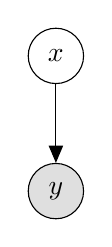
\begin{tikzpicture}

\node[obs](y){$y$};
% Define nodes
\node[latent, above= of y, xshift=0cm]   (x) {$x$}; 

% Connect the nodes
\edge {x} {y} ; %

% Plates
%\plate {yx} {(x)(y)} {$N$} ;
%\plate {} {(w)(y)(yx.north west)(yx.south west)} {$M$} ;

\end{tikzpicture}
%\endpgfgraphicnamed

%%% Local Variables: 
%%% mode: tex-pdf
%%% TeX-master: "example"
%%% End: 
	\end{center}
	\caption{The FOPPL code for the conditional Gaussian}
\end{figure}
This model has the following joint $ p(x,y) \propto p(x|y) = p(x)p(y| x) = \mathcal{N}(\bar{\mu}, \bar{\sigma}^{2})$, where $\bar{\mu} = \left(\frac{\mu_{0}\sigma^{2} + \sigma^{2}_{0}\sum_{i=1}^{n}y_{i}}{\sigma^{2}\sigma^{2}_{0}}\right) \bar{\sigma}^{2}$ and $\bar{\sigma}^{2} = \left(\frac{1}{\sigma^{2}_{0}} + \frac{n}{\sigma^{2}}\right)^{-1} $. In this model, $n$ is the total number of observed datum $y$, $\mu_{0} = 0 $ and $\sigma_{0}^{2} = 1$ are the prior mean and variance and $\sigma^{2} = 1.0 $ is the likelihood variance. Thus, the true mean that our model should infer is $\bar{\mu} = 5$. This is indeed the value that we get as can be seen via figures(\ref{fig:plotconj1}-\ref{fig:plotconj3}).
\subsubsection{Conditional If}
\begin{figure}[ht]
	\label{fig:conif}
	\begin{center}
		% !tex root=/main.tex
\beginpgfgraphicnamed{conif}
\begin{tikzpicture}

% Define nodes
\node[obs, xshift = -2cm]   (y2){$y$};
\node[obs, xshift = 0cm] (y1){$y$};
\node[det, above= of {y1, y2}, xshift = -1cm ]     (if) {if-else} ; % 
\node[latent, above= of if]             (x){$x$};
%\node[latent, above= of y, xshift=0cm]   (true) {$z_{n}$};
%\node[latent, above=of z, xshift=0cm]   (false) {$s$};
%\node[latent, above=of z, xshift=1.2cm]  (b) {$b$};
%\node[obs, above= of z, xshift=-1.2cm]   (x) {$x_{n}$}; 

% Connect the nodes
\edge {x}{if};
\edge [dashed]{if}{y1,y2};

% Plates
%\plate {yx} {(x)(y)} {$N$} ;
%\plate {} {(w)(y)(yx.north west)(yx.south west)} {$M$} ;

\end{tikzpicture}
	\end{center}
	\caption{Conditional if graphical model}
\end{figure}
The conditional \mintinline{clojure}{if} statement, see figure (\ref{fig:conif})is typically challenging to implement for gradient based methods, due to the branching effects that occur at the condition. For trace based samplers, such as importance sampling, this is not a problem as multiple traces are recorded for each path taken. However, in higher dimensions these types of samplers are heavily impaired, which is why we need additional MCMC methods to be able to perform efficiently in in higher dimensions. In FOPPL we would write a simple conditional \mintinline{clojure}{if} program as follows:\inputminted{clojure}{code/conditionalif.clj}
 In this model, we have a joint distribution of the form $p(x,y) \propto p(x|y) = \mathcal{N}(0,1)\mathcal{N}(y = 1|1,1)^{\mathbb{I}(x > 0)}\mathcal{N}(y = 1|-1,1)^{\mathbb{I}(x < 0)}$, where $\mathbb{I}(\cdot)$ represents the indicator function. The empirical mean that we generate for this model is 0.58 and if you plot the unnormalized joint, the shape is the same, but the density values are of course different, see figures (\ref{fig:plotif1}-\ref{fig:plotif3}). This implies that we can be confident in the results generated by the HMC.
% If we are to analytically calculate the mean, we have to look at the case where $x < 0$ and the case where $x>0$. Using the sum rule the evidence can be found by $p(y) = \int p(x,y) dx $, which we analytically calculate to be, $p_{x<0}(y) = -\mathcal{N}(y=1|-1,1)\sqrt{2\pi}$ and for $x>0$ we have  $p_{x>0}(y) = \mathcal{N}(y=1| 1,1)\sqrt{2\pi}$. Thus, by Bayes rule, the full posterior is given as $p(x | y) = \frac{p(y|x)p(x)}{p(y)} = \frac{\mathcal{N}(0,1)\mathcal{N}(y = 1|1,1)^{\mathbb{I}(x > 0)}\mathcal{N}(y = 1|-1,1)^{\mathbb{I}(x < 0)}}{\sqrt{(2\pi)(\mathcal{N}(y = 1|-1,1)^{\mathbb{I}(x < 0)} + \mathcal{N}(y = 1|1,1)^{\mathbb{I}(x > 0)} )}}$ .    
\subsubsection{Linear Regression}
\begin{figure}[ht]
	\label{fig:lrgraph}
	\begin{center}
		% model_pca.tex
%
% Copyright (C) 2012 Jaakko Luttinen
%
% The MIT License
%
% See LICENSE file for more details.

% PCA model

%\beginpgfgraphicnamed{model-pca}
%\begin{tikzpicture}
%
%  % Define nodes
%  \node[obs]                               (y) {$y$};
%  \node[latent, above=of y, xshift=-1.2cm] (w) {$\mathbf{w}$};
%  \node[latent, above=of y, xshift=1.2cm]  (x) {$\mathbf{x}$};
%  \node[latent, right=2cm of y]            (t) {$\tau$};
%
%  % Connect the nodes
%  \edge {x,w,t} {y} ; %
%
%  % Plates
%  \plate {yx} {(x)(y)} {$N$} ;
%  \plate {} {(w)(y)(yx.north west)(yx.south west)} {$M$} ;
%
%\end{tikzpicture}
%\endpgfgraphicnamed

%%% Local Variables: 
%%% mode: tex-pdf
%%% TeX-master: "example"
%%% End: % model_pca.tex
%
% Copyright (C) 2012 Jaakko Luttinen
%
% The MIT License
%
% See LICENSE file for more details.

% PCA model

%\beginpgfgraphicnamed{model-pca}
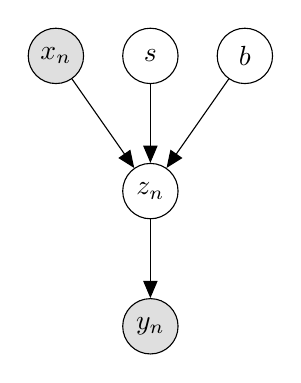
\begin{tikzpicture}

\node[obs](y){$y_{n}$};
% Define nodes
\node[latent, above= of y, xshift=0cm]   (z) {$z_{n}$};
\node[latent, above=of z, xshift=0cm]   (s) {$s$};
\node[latent, above=of z, xshift=1.2cm]  (b) {$b$};
\node[obs, above= of z, xshift=-1.2cm]   (x) {$x_{n}$}; 

% Connect the nodes
\edge {x,s,b} {z} ; %
\edge {z} {y} ;

% Plates
%\plate {yx} {(x)(y)} {$N$} ;
%\plate {} {(w)(y)(yx.north west)(yx.south west)} {$M$} ;

\end{tikzpicture}
%\endpgfgraphicnamed

%%% Local Variables: 
%%% mode: tex-pdf
%%% TeX-master: "example"
%%% End: 
	\end{center}
	\caption{Linear regression model as a graph.}
\end{figure}
In this problem we have a set of points $\{(x,y)\}$ and we wish to infer the equation of a line in a Bayesian manner, such that the line goes through all of those points. See figure (\ref{fig:lrgraph}) for a graphical model of the model. To do this, we must infer the slope and the bias of the line, which is done by placing priors on our parameters of interest and observations. The FOPPL program corresponding to figure (\ref{fig:lrgraph}) can be written as follows: \inputminted{clojure}{code/linearregression.clj}.In this model for both the slope and bias, we \mintinline{clojure}{sample} from $\mathcal{N}(0,10.0)$ and we state that likelihood of the model is of the form of a conditional Gaussian $\mathcal{N}(y_{n}| z_{n}, 1.0)$ with a mean dependent on our sampled line.   Therefore, we can construct the joint for this model as follows: 
$p(x_{n},s,b,z_{n}, y_{n}) \propto p(s,b,z_{n} | x_{n}, y_{n}) = p(s)p(b)p(y | z_{n}, 1) =\mathcal{N}(0,5^{2})\mathcal{N}(y_{n}|z_{n},1.0)$. We can analytically calculate the equation of a straight line by using the formula $\left(\frac{y - y_{*}}{x - x_{*}}\right) = m$, which leads to $y = mx + b$. From this we find that the true slope $m = 1.6$ and the bias $b = 0.5$. We again see from figures \ref{fig:plotlr1}-\ref{fig:plotlr3}, that the HMC correctly calculates the true values of the parameters.\\
	
\subsection{Experimental Results}
	\begin{figure*}[ht]
	\centering
	\subcaptionbox{\label{fig:plotconj1}}[.3\linewidth][c]{%
		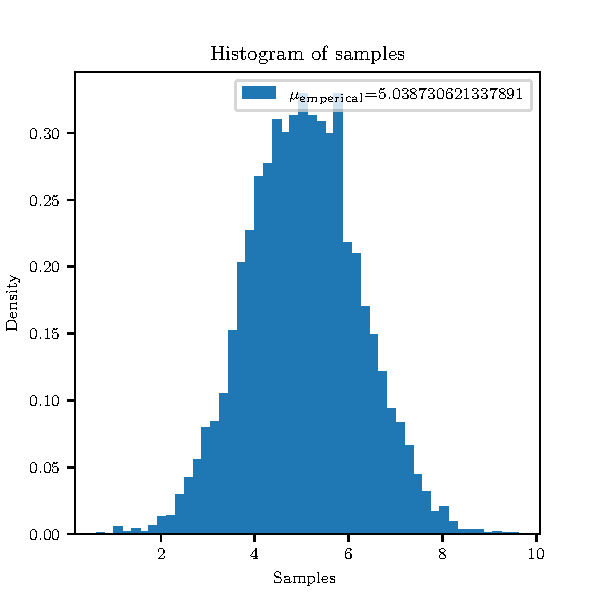
\includegraphics[width=.2\linewidth]{conjgauss/figures/histogram.pdf}}\quad
	\subcaptionbox{}[.3\linewidth][c]{%
		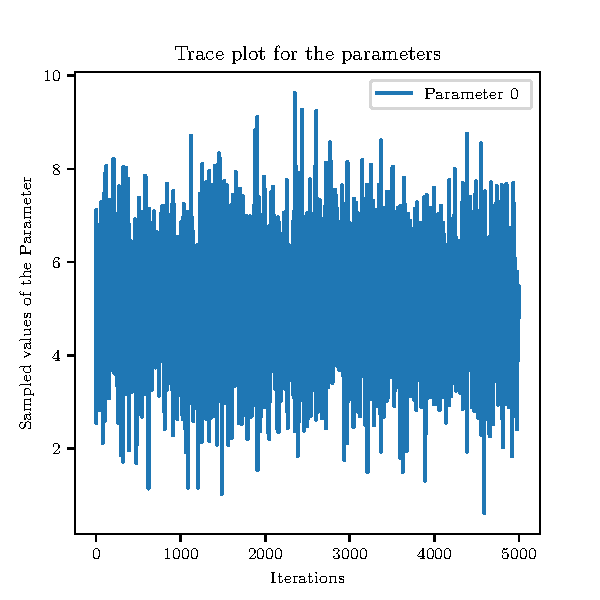
\includegraphics[width=.2\linewidth]{conjgauss/figures/trace.pdf}}\quad
	\subcaptionbox{\label{fig:plotconj3}}[.3\linewidth][c]{%
		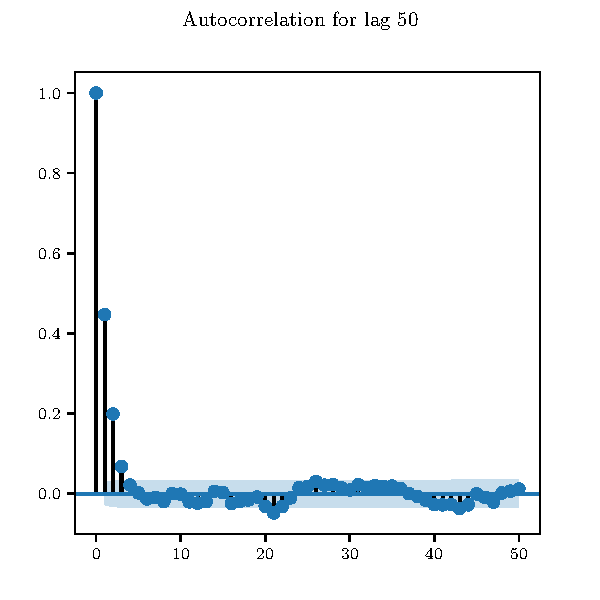
\includegraphics[width=.2\linewidth]{conjgauss/figures/Autocorrelationplot.pdf}}
	
	\bigskip
	\subcaptionbox{	\label{fig:plotif1}}[.3\linewidth][c]{%
		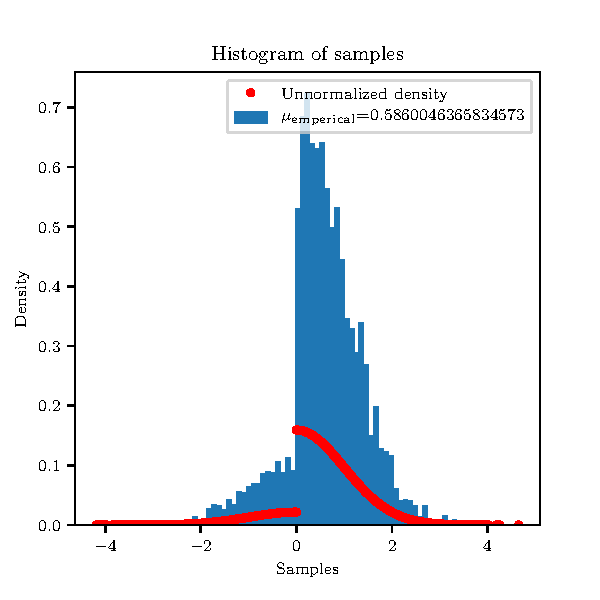
\includegraphics[width=.2\linewidth]{conditionalif/figures/histogram_with_density.pdf}}\quad
	\subcaptionbox{}[.3\linewidth][c]{%
		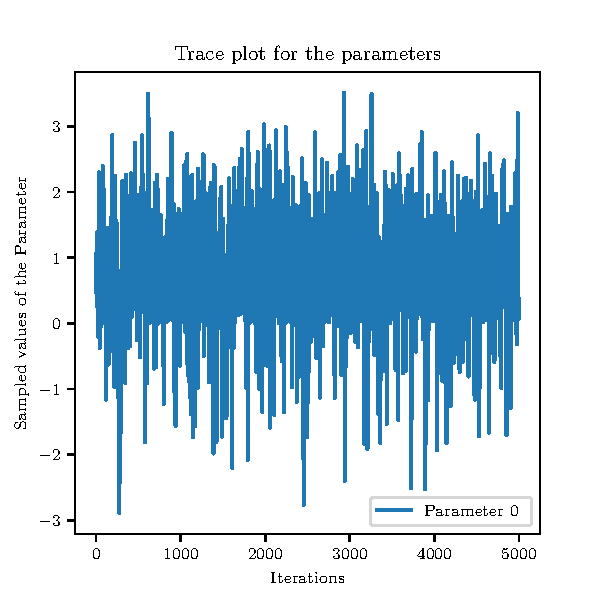
\includegraphics[width=.2\linewidth]{conditionalif/figures/trace.pdf}}\quad
	\subcaptionbox{	\label{fig:plotif3}}[.3\linewidth][c]{%
		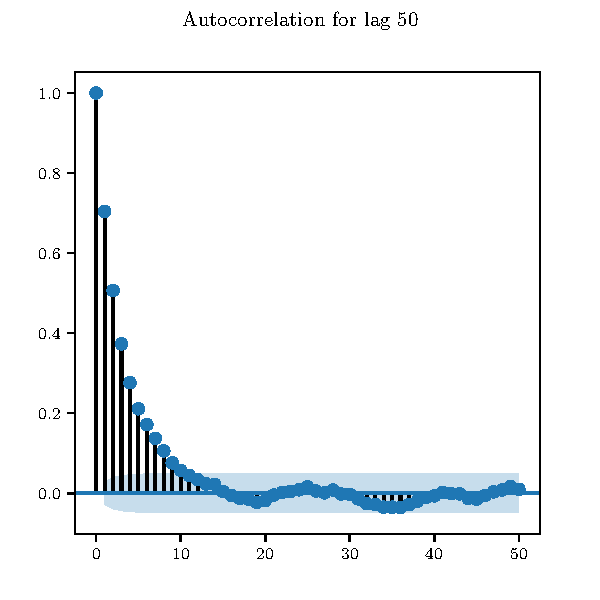
\includegraphics[width=.2\linewidth]{conditionalif/figures/Autocorrelationplot.pdf}}
	
	\bigskip
    \subcaptionbox{	\label{fig:plotlr1} }[.3\linewidth][c]{%
		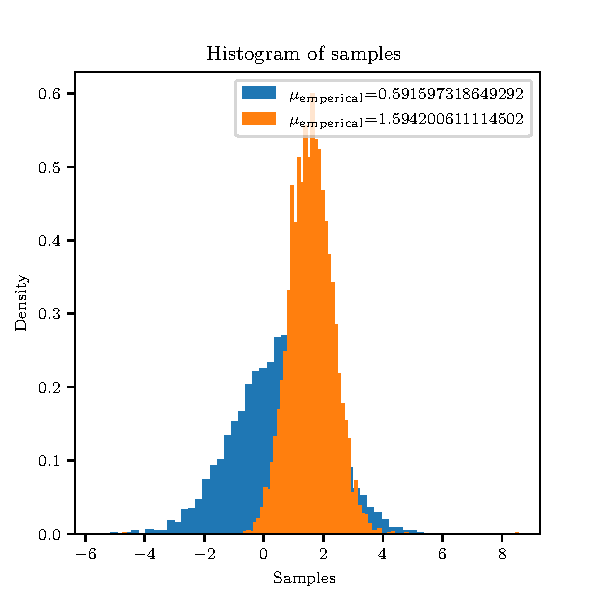
\includegraphics[width=.2\linewidth]{linearreg/figures/histogram.pdf}}\quad
	\subcaptionbox{}[.3\linewidth][c]{%
		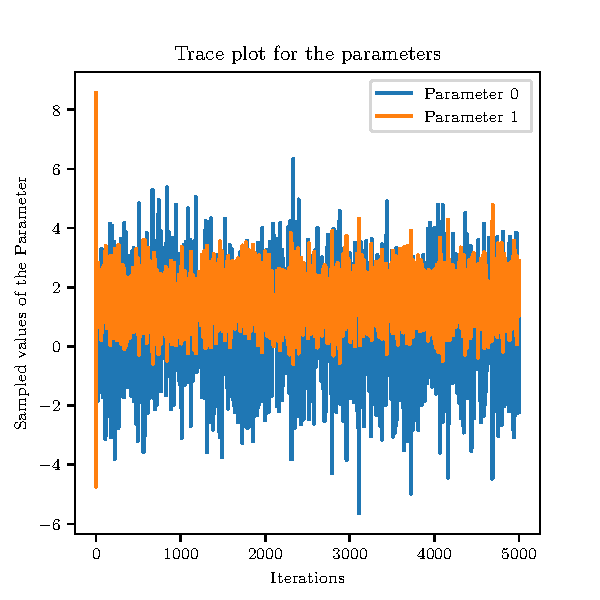
\includegraphics[width=.2\linewidth]{linearreg/figures/trace.pdf}}\quad
	\subcaptionbox{	\label{fig:plotlr3}Left: bias . Right: slope.}[.3\linewidth][c]{%
		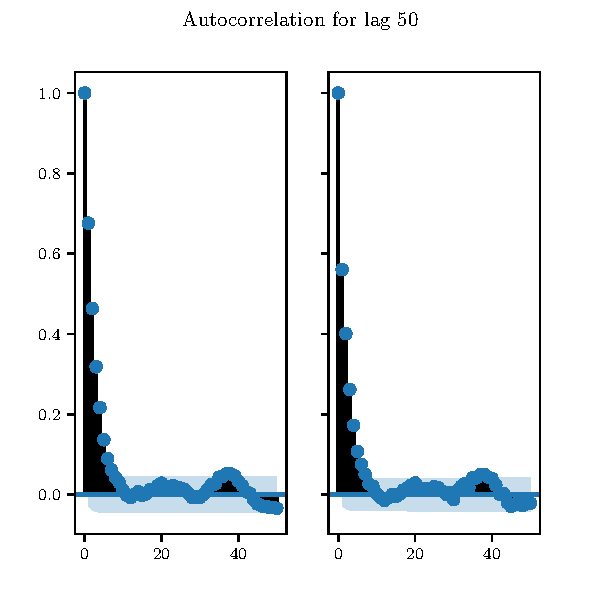
\includegraphics[width=.2\linewidth]{linearreg/figures/Autocorrelationplot.pdf}}
	\caption{Each row corresponds to the inference output of each model and provides a histogram of the samples, the trace of the samples for each parameter of interest in the model and the autocorrelation between the samples for a lag $l = 50$. \textit{Top row} represents the conjugate Gaussian model,\textit{Middle row} represents the conditional if model. \textit{Bottom row} represents the linear regression model with parameter 0, in blue, representing the bias and parameter 1, in orange, represents the slope of the line.  }
	\end{figure*}

\section{Discussion}
%Fourth level headings must be flush left, initial caps, bold, and
%Roman type.  Use one line space before the fourth level heading, and
%place the section text immediately after the heading with no line
%break, but an 11 point horizontal space.

%\subsection{CITATIONS, FIGURES, REFERENCES}
%
%
%\subsubsection{Citations in Text}
%
%%Citations within the text should include the author's last name and
%%year, e.g., (Cheesman, 1985). References should follow any style that
%%you are used to using, as long as their style is consistent throughout
%%the paper.  Be sure that the sentence reads correctly if the citation
%%is deleted: e.g., instead of ``As described by (Cheesman, 1985), we
%%first frobulate the widgets,'' write ``As described by Cheesman
%%(1985), we first frobulate the widgets.''  %Be sure to avoid
%%%accidentally disclosing author identities through citations.
%
%\subsubsection{Footnotes}
%
%%Indicate footnotes with a number\footnote{Sample of the first
%%  footnote.} in the text. Use 8 point type for footnotes. Place the
%%footnotes at the bottom of the column in which their markers appear,
%%continuing to the next column if required. Precede the footnote
%%section of a column with a 0.5 point horizontal rule 1~inch (6~picas)
%%long.\footnote{Sample of the second footnote.}
%
%\subsubsection{Figures}


%Make sure that the figure caption does not get separated from the
%figure. Leave extra white space at the bottom of the page rather than
%splitting the figure and figure caption.
%\begin{figure}[ht]
%	\vspace{.3in}
%	\centering
%	\includegraphics[width=.3\textwidth]{weierstrass_si_small/resized002.png}\quad
%	\includegraphics[width=.3\textwidth]{weierstrass_si_small/resized003.png}
%	\vspace{.3in}
%	\caption{A prediction of the Weierstrass on 20\% of the data set, 200 pts, in the single-input model. The top row is a linear combination of covariance functions operating on the original observations. The middle row represents the prediction, the posterior mean is in green, the observables are in red and the targets are in blue. The bottom row is the posterior covariance at the levels 0 and 4.}
%	\label{pics:si_wie_s}
%\end{figure}
%\begin{figure}[h]
%\vspace{.3in}
%\centerline{\fbox{This figure intentionally left non-blank}}
%\vspace{.3in}
%\caption{Sample Figure Caption}
%\end{figure}
%
%\subsubsection{Tables}
%
%All tables must be centered, neat, clean, and legible. Do not use hand-drawn tables. Table number and title always appear above the table.
%See Table~\ref{sample-table}.
%
%Use one line space before the table title, one line space after the table title, and one line space after the table. The table title must be
%initial caps and each table numbered consecutively.
%
%%\begin{table}
%%\caption{Sample Table Title} \label{sample-table}
%%\begin{center}
%%\begin{tabular}{ll}
%%{\bf PART}  &{\bf DESCRIPTION} \\
%%\hline \\
%%Dendrite         &Input terminal \\
%%Axon             &Output terminal \\
%%Soma             &Cell body (contains cell nucleus) \\
%%\end{tabular}
%%\end{center}git 
%%\end{table}

\section{Supplementary Material}
\label{sec:supmat}

In the supplementary material we show some examples of the compiler output for the linear regression and conjugate Gaussian models. We also discuss the implementation of the HMC algorithm itself in pytorch and state how we have intertwined both the inference and FOPPL. As the FOPPL program produces an actual directed graph as output, like the ones seen in section \ref{sec:exampprog},  we must take that structure and map the edges, vertices and nodes accordingly into the right model output. This means that we must take care to ensure that the structure of language specific statements such as \mintinline{clojure}{observe}, \mintinline{clojure}{sample}, \mintinline{clojure}{let, defn, if} and language grammar such as \mintinline{clojure}{variable, constant, procedure}. 
\inputminted{python}{code/cjgauss.py}
\inputminted{python}{code/lr_out.py}
\inputminted{python}{code/hmc_class.py}
\inputminted{python}{code/cjgauss.py}
%\section{INSTRUCTIONS FOR CAMERA-READY PAPERS}

%For the camera-ready paper, if you are using \LaTeX, please make sure
%that you follow these instructions.  (If you are not using \LaTeX,
%please make sure to achieve the same effect using your chosen
%typesetting package.) Blah blah

%\begin{enumerate}
%    \item Download \texttt{fancyhdr.sty} -- the
%    \texttt{aistats2017.sty} file will make use of it.
%    \item Begin your document with
%    \begin{flushleft}
%    \texttt{\textbackslash documentclass[twoside]\{article\}}\\
%    \texttt{\textbackslash usepackage[accepted]\{aistats2017\}}
%    \end{flushleft}
%    The \texttt{twoside} option for the class article allows the
%    package \texttt{fancyhdr.sty} to include headings for even and odd
%    numbered pages. The option \texttt{accepted} for the package
%    \texttt{aistats2017.sty} will write a copyright notice at the end of
%    the first column of the first page. This option will also print
%    headings for the paper.  For the \emph{even} pages, the title of
%    the paper will be used as heading and for \emph{odd} pages the
%    author names will be used as heading.  If the title of the paper
%    is too long or the number of authors is too large, the style will
%    print a warning message as heading. If this happens additional
%    commands can be used to place as headings shorter versions of the
%    title and the author names. This is explained in the next point.
%    \item  If you get warning messages as described above, then
%    immediately after $\texttt{\textbackslash
%    begin\{document\}}$, write
%    \begin{flushleft}
%    \texttt{\textbackslash runningtitle\{Provide here an alternative shorter version of the title of your
%    paper\}}\\
%    \texttt{\textbackslash runningauthor\{Provide here the surnames of the authors of your paper, all separated by
%    commas\}}
%    \end{flushleft}
%    Note that the text that appears as argument in \texttt{\textbackslash
%      runningtitle} will be printed as a heading in the \emph{even}
%    pages. The text that appears as argument in \texttt{\textbackslash
%      runningauthor} will be printed as a heading in the \emph{odd}
%    pages.  If even the author surnames do not fit, it is acceptable
%    to give a subset of author names followed by ``et al.''
%
%    \item Use the file sample\_paper.tex as an example.
%
%    \item The camera-ready versions of the accepted papers are 8
%      pages, plus any additional pages needed for references.
%
%    \item If you need to include additional appendices,
%      you can include them in the supplementary
%      material file.
%
%    \item Please, don't change the layout given by the above
%      instructions and by the style file.
%
%\end{enumerate}

\subsubsection*{Acknowledgements}

Use unnumbered third level headings for the acknowledgements.  All
acknowledgements go at the end of the paper.

\subsubsection*{References}
\bibliographystyle{apalike}
\bibliography{mini_proj}


\end{document}
